\chapter{Automatização de processos}\label{chp:automatizacao_processos}

\section{Processos}\label{sec:automatizacao_processos-processos}
Processo de negócio é um conjunto de atividades coordenadas, relacionadas entre si, que envolvem diferentes pessoas, procedimentos, áreas e tecnologias com o objetivo de gerar valor para a empresa, seja em forma de produtos ou serviços, internos ou externos.

\section{BPM}\label{sec:automatizacao_processos-bpm}
BPM é o acrônimo para o inglês Business Process Management, ou gestão de processos de negócio, em português. Seu principal objetivo é oferecer uma abordagem sistemática para a execução, adaptação e melhoria de processos de negócio em um ambiente de constantes mudanças. O BPM pode ser encarado sob duas perspectivas distintas: o BPM como engenharia de software ou o BPM como disciplina de gestão.

\section{BPMN}\label{sec:automatizacao_processos-bpmn}
A BPMN (Business Process Management Notation, em português, notação de gerenciamento de processos de negócio) foi criada para representar processos de negócio em forma de diagrama, através de uma notação padronizada e de fácil entendimento por diferentes profissionais, sejam desenvolvedores, analistas de negócio ou gestores. Foi criada inicialmente pelo BPMI (Business Process Management Initiative) em 2004, mas atualmente é mantida e atualizada pela OMG (Object Management Group). Sua versão mais atual é a BPMN 2.0, publicada em 2011.

A notação foi concebida sob a perspectiva de cobrir a falta de entendimento entre diferentes departamentos e organizações a cerca de um determinado processo ou conjunto de processos, algo muito frequente no ambiente corporativo. Além disso, através de sua notação padronizada em XML (Extensible Markup Language), diferentes ferramentas podem fazer o uso de sua auto-descrição para automatizar a orquestração de processos de negócio.

\begin{figure}[H]
  \centering
  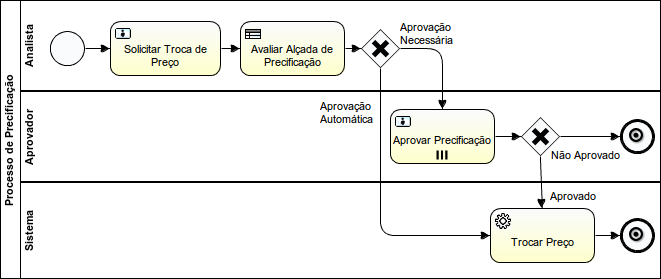
\includegraphics[width=1.0\textwidth]{imagens/ProcessoDePrecificacao.png}
  \caption{Processo representado em BPMN}
  \label{fig:exemplo_bpmn}
\end{figure}

\subsection{Objetos}\label{sec:automatizacao_processos-bpmn_objetos}

A notação define quatro grupos distintos de objetos para permitir a diagramação de um fluxo de negócio. Os objetos são classificados em artefatos, agrupadores, conectores e objetos de fluxo. São utilizadas figuras geométricas, como retângulos e círculos, além de linhas pontilhadas e tracejadas, entre outros elementos para representar cada um dos objetos que constituem a notação.

\subsubsection{Objetos de Fluxo}\label{sec:automatizacao_processos-bpmn_objetos_fluxo}

Os objetos de fluxo são os principais elementos do BPMN pois constiuem os elementos chave na execução do fluxo de trabalho.


\begin{enumerate}
    \item Eventos
    
    Objetos utilizados para representar que algo "aconteceu" durante a execução do fluxo. São exemplos de eventos: "chamada de sistema externo recebida", "envio de cancelamento do processo recebido", "a cada 1 minuto". A notação BPMN 2.0 define mais de 60 tipos distintos de eventos.
    
    \begin{figure}[H]
    \centering
    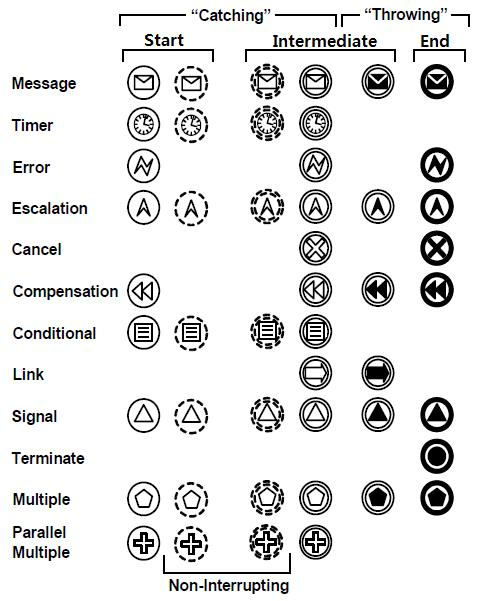
\includegraphics[width=0.65\textwidth]{imagens/bpmn_events.jpg}
    \caption{Tipos de Eventos}
    \label{fig:bpmn_events}
    \end{figure}
    
    \item Atividades
    
    Objetos utilizados para representar uma unidade de trabalho a ser realizada no processo. Existem dois tipos básicos de atividades: tarefas ou subprocessos. As tarefas podem ser executadas por humanos ou por algum tipo de serviço, como um seviço web ou mesmo a execução de algum código interno no processo.
    
    \begin{figure}[H]
    \centering
    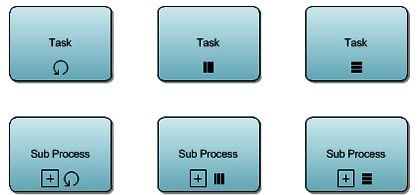
\includegraphics[width=0.55\textwidth]{imagens/bpmn_activities.jpg}
    \caption{Tipos de Atividades}
    \label{fig:bpmn_activities}
    \end{figure}
    
    \item Decisões
    
    São objetos utilizados para controlar o fluxo de trabalho, possibilitando o direcionamento do processo para a escolha de único sentido, ou para controlar a divergência e convergência de fluxos paralelos.
    
    \begin{figure}[H]
    \centering
    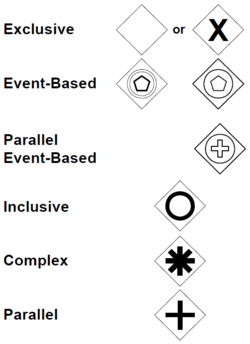
\includegraphics[width=0.4\textwidth]{imagens/bpmn_gateways.png}
    \caption{Tipos de Decisões}
    \label{fig:bpmn_gateways}
    \end{figure}
\end{enumerate}


\subsubsection{Agrupadores}\label{sec:automatizacao_processos-bpmn_objetos_agrupadores}

    São objetos utilizados para organizar visualmente a distribuição dos demais objetos do processo em contêineres que representam a responsabilidade de determinado ator do processo.

    \begin{figure}[H]
    \centering
    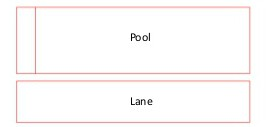
\includegraphics[width=0.5\textwidth]{imagens/bpmn_swimlanes.jpg}
    \caption{Tipos de Agrupadores}
    \label{fig:bpmn_swimlanes}
    \end{figure}

\subsubsection{Conectores}\label{sec:automatizacao_processos-bpmn_objetos_conectores}

    São utilizados para interligar objetos de fluxo. São classificados em conectores de sequência, mensagem ou associação.

    \begin{figure}[H]
    \centering
    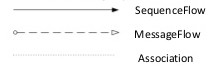
\includegraphics[width=0.5\textwidth]{imagens/bpmn_connectors.jpg}
    \caption{Tipos de Conectores}
    \label{fig:bpmn_conectors}
    \end{figure}

\subsubsection{Artefatos}\label{sec:automatizacao_processos-bpmn_objetos_artefatos}

    São utilizados para acrescentar informações adicionais a modelagem do processo. 

    \begin{figure}[H]
    \centering
    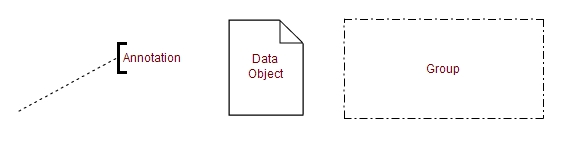
\includegraphics[width=0.8\textwidth]{imagens/bpmn_artifacts.jpg}
    \caption{Tipos de Artefatos}
    \label{fig:bpmn_artifacts}
    \end{figure}

\section{BPMS}\label{sec:automatizacao-processos-bpms}
\subsection{Activiti BPM}\label{sec:automatizacao-processos-bpms-activiti}
\subsection{Bonita}\label{sec:automatizacao-processos-bpms-bonita}
\subsection{jBPM}\label{sec:automatizacao-processos-bpms-jbpm}
\subsection{Intalio}\label{sec:automatizacao-processos-bpms-intalio}
